\documentclass[a4paper,twoside]{articlek}
\newcommand{\mins}{&\!\!\!\!}
\renewcommand{\refname}{REFERENCES}
\textwidth=17.3truecm \hoffset=0.55truecm \textheight=26.4truecm
\topmargin=-2.2truecm \columnsep=0.7truecm \oddsidemargin =
-.4truecm \evensidemargin = -1.7truecm \pagenumbering{arabic}
\pagestyle{headings} \setcounter{page}{0}
\newlength{\sectionName}
\newlength{\sectionNameP}
\unitlength=1cm
\frenchspacing
%\parindent=0cm
\def\be{\begin{equation}}
\def\ee{\end{equation}}
% ------------------------------------------------------------------------

\def\BibTeX{{\rm B\kern-.05em{\sc i\kern-.025em b}\kern-.08em
            T\kern-.1667em\lower.7ex\hbox{E}\kern-.125emX}}

\usepackage[utf8x]{inputenc}
\usepackage{graphicx}
% ------------------------------------------------------------------------
\begin{document}
\sloppy
\twocolumn[{
%\vspace*{1.7cm}   % for the title  page only
%\begin{center}
{\large\bf INTERFEROMETRIC PLASMA DENSITY MEASUREMENT IN GOLEM TOKAMAK}\\

	{\small %A. Author, e-mail, B. Author, e-mail, address and C.
O. Grover, ondrej.grover@gmail.com, FJFI ČVUT (Cesta k Vědě)}\\ %TODO what address and other authors included ?

%\end{center}
%\vspace*{1ex}

%{\bf ABSTRACT.} These are the guidelines for preparation of
%manuscripts of the contributions to the proceedings of the 17th
%Conference of Czech and Slovak Physicists, held on September 5 -
%8, 2011.\\
}]
\section{INTRODUCTION}
Electron density is on of the key parameters in the field of plasma physics. Its measurement provides important information about the behaviour and characteristics of plasma. For that purpose many different methods of density measurement exist.% yoda
The most widespread are microwave diagnostics, mainly because of their non-invasive nature. 

The microwave interferometer which has been recently installed at the GOLEM Tokamak measures the line-averaged electron density and can be used to track the time evolution during a discharge.%time evolution\ldots term?
This diagnostic had been previously implemented on the same device when it was in service as the CASTOR Tokamak %reformulate 
at the Czech Academy of Sciences and the whole waveguide system and other analytical hardware were made with the specific parameters of the site and work-flow in mind. This paper presents the current state of implementation at the GOLEM Tokamak.

\section{FUNDAMENTAL PRINCIPLES OF OPERATION} % find something better and CAPS

In ionized plasma oscillations of electrons around ions arise when the homogeneity of the electrostatic charge is disrupted. The angular frequency of such plasma oscillations $\omega_p$ is dependant on the electron density $n_e$. 

As shown in \cite{mateju}, an electromagnetic wave propagating through plasma perpendicularly to the magnetic and electric field\footnote{a so called ``ordinary wave'', the geometry of a conventional Tokamak allows for such fields to exist} has a dispersion relation
\begin{equation}
    \omega = \omega_p +c^2 k^2
    \label{eq:dispersion}
\end{equation}
where $\omega$ is the angular frequency of the propagating EM wave, $k$ is its wavenumber and $c$ is the speed of light in vacuum.

Therefore an EM wave with a given angular frequency $\omega>\omega_p$ has a real wavenumber $k$ and it propagates with a phase velocity $v_p>c$. Hence the refractive index $n$ is less than 1 and is dependent on $\omega_p$, thus also dependent on the electron density $n_e$. 

As $\omega$ approaches $\omega_p$, the refractive index $n$ approaches 0 so the EM wave cannot propagate and is reflected. Thus for probing beam with a given $\omega$ there is a so called critical density $n_{crit}$ above which the measurement cannot take place.


A microwave beam probing the plasma undergoes a phase shift $\Delta \varphi$ due to the different $n$.  %or is it not ? REFORMULATE
As $n_e$ and therefore also $n$ differs throughout the plasma, the total phase shift is directly proportional to the line integral of $n_e$ over the distance $d$ traveled through plasma as has been derived in \cite{mateju}
\begin{equation}
    \overline{n_e}=\frac{ n_{crit}\lambda_0 }{d \pi}\Delta \varphi
    \label{eq:ne}
\end{equation}
where $\lambda_0$ is the wavelength of the microwave in vacuum and $d$ is the distance that the microwave beam travels through plasma. 

$\Delta \varphi$ is then extracted from the interference of the probing MW beam and the reference beam which was split off from the probing beam before entering plasma and thus has the same phase as the probing beam had before it entered plasma.

\section{FREQUENCY MODULATION}

The Gunn diode MW generator generates microwaves with frequencies $f \sim 75$ GHz. Analyzing the interference and extracting the phase shift at such high frequencies would be a very hard task and the time resolution obtained by analysing such high frequencies would be unnecessary as it it assumed that the density of plasma doesn't change as quickly.

Therefore, frequency modulation is used to scale down the time resolution of the analyzed signal. The frequency $f$ of the microwaves generated by the Gunn diode can be scaled by applying external voltage. There is also a difference $\Delta L$ between the distance traveled by the reference wave and the probing wave as the reference wave travels several centimeters from the generator directly to the mixer diode where it interferes with the probing wave which had to travel several meters from the generator, to the chamber and back to the mixing diode.

This design results in beats when the two waves interfere, provided the frequency of the generated MWs is progressively scaled, because the waves will have different frequencies due to the difference in distances. 

Ideally, $f$ would be continuously linearly scaled up with a rate of change $\frac{df}{dt}$ which would result in a constant difference $f_{diff}$ between the frequencies of the waves 
\begin{equation}
f_{diff}=\frac{\Delta L}{c} \frac{df}{dt}
\label{eq:fdiff}
\end{equation}
 Therefore, $f_{diff}$ would be also the frequency of the absolute value of the amplitude of the beats.

However, the generated frequency can be scaled up only to a certain level, therefore the linear scaling slope has to be broken down to a periodic saw-tooth slope with an amplitude $\Delta f$ and a frequency $f_{mod}$.

From (\ref{eq:fdiff}) it can be derived that while 
\begin{equation}
\Delta f=\frac{c}{\Delta L}
\label{eq:Df}
\end{equation}

it is true that $f_{mod}=f_{diff}$ and thus the frequency of the resulting beats can be controlled by applying a saw-tooth voltage signal with the right parameters to the generator. 

The beat interference is then processed by a selective frequency band amplifier which amplifies signals with frequencies $500 \pm 20$ kHz. Therefore, the parameters of the saw-tooth voltage signal are $f_{mod}=500$ kHz and $\Delta L$ is set for (\ref{eq:Df}) to be true.

\section{WAVEGUIDE SYSTEM}
\begin{figure}[b]
    \begin{center}
        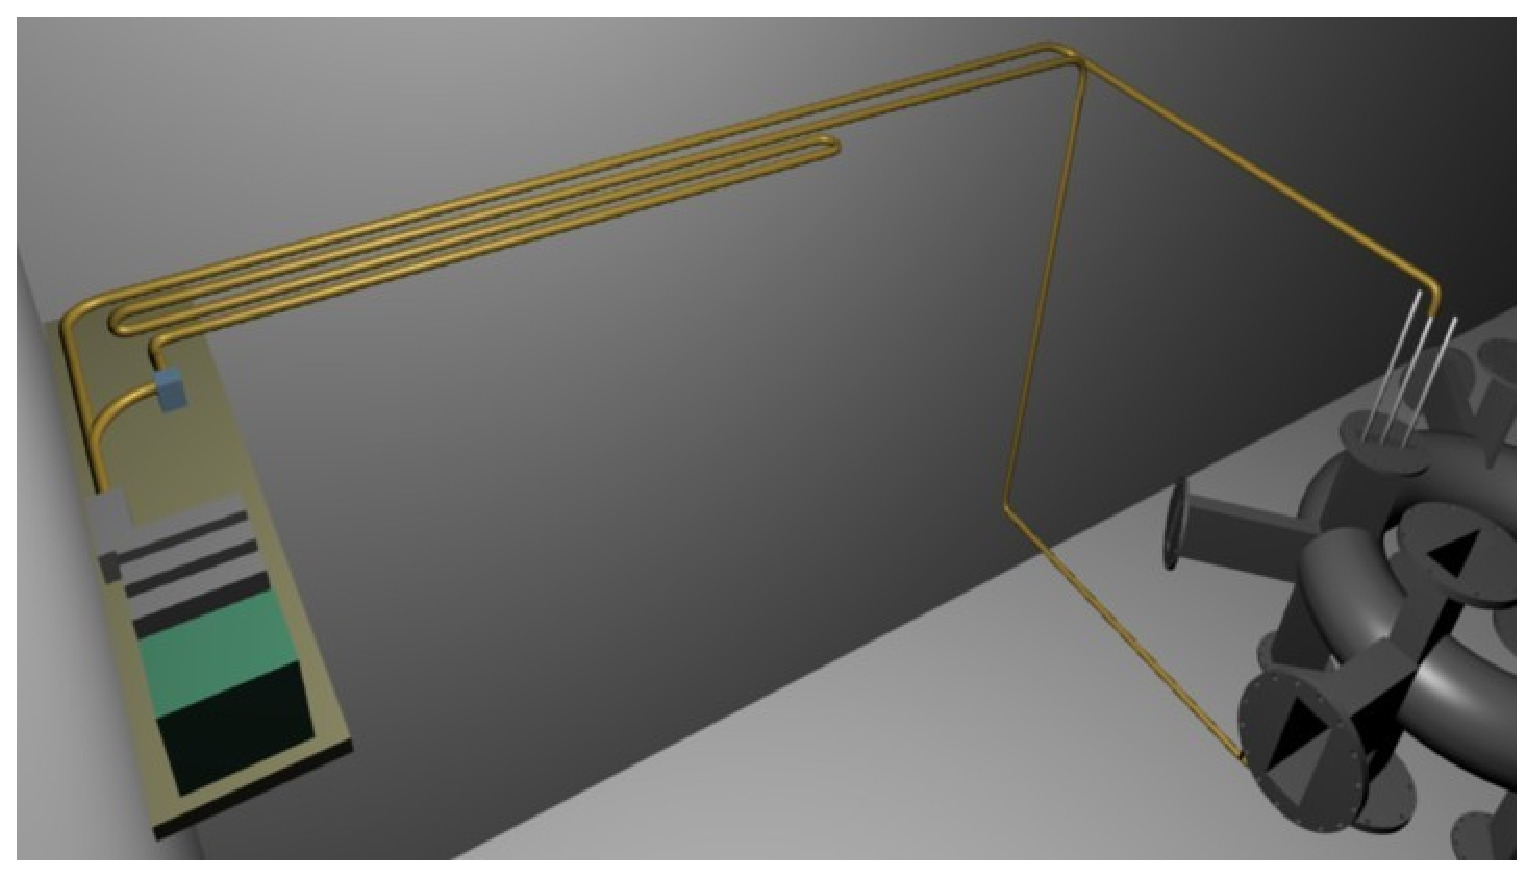
\includegraphics[width=.45\textwidth]{vlnovody.eps}
    \end{center}
    \caption{3D model of the new waveguide system}
    \label{fig:ws}
\end{figure}
All the diagnostic hardware including the amplifier and the generator were designed to work with the waveguide system as it was constructed at the Czech Academy of Sciences for the CASTOR tokamak, so the band of the amplifier is fixed and $\Delta f$ can be set only within a certain range.

Therefore, the new waveguide system had to have approximately the same length as the old one (about 12 m) and at the same time fit into the modest room where the GOLEM tokamak is today located. 
This was achieved by constructing several U-turns resulting in a ``trombone-like'' design as seen in Figure \ref{fig:ws}.

\section{METHODS OF SIGNAL ANALYSIS}

The output of the amplifier is a sine wave signal with a frequency $f_{mod}$. The phase shift can be extracted from it by either an analogue analysis circuit or digitally by first digitizing the signal with a Tektronix DPO 3014 oscilloscope and then processing on a computer. 

The analogue circuit measures the time between the trigger signal and the roots of the sine signal. The trigger signal is synchronously generated by saw-tooth voltage generator with $f_{mod}$. However, the circuit compares only every eighth trigger signal, thus the sampling frequency of this method is only $62,5$ kHz. The output of the circuit is voltage directly proportional to $\Delta \varphi $, 1V$\sim 2\pi$. This output is digitized and then processed with (\ref{eq:ne}).

The oscilloscope digitizes the signal with a sampling f. of 25 MHz. The data is then filtered for regions where the amplitude is close to 0, because there the amplitude dampening is assumed to be minimal. These regions are then fitted to $f(t)=A\sin(2 \pi 5e5 t+ \varphi)$ and the fitted value of $\varphi$ is further processed with (\ref{eq:ne}).

\section{SIGNAL DISTURBANCES}
\begin{figure}
    \begin{center}
        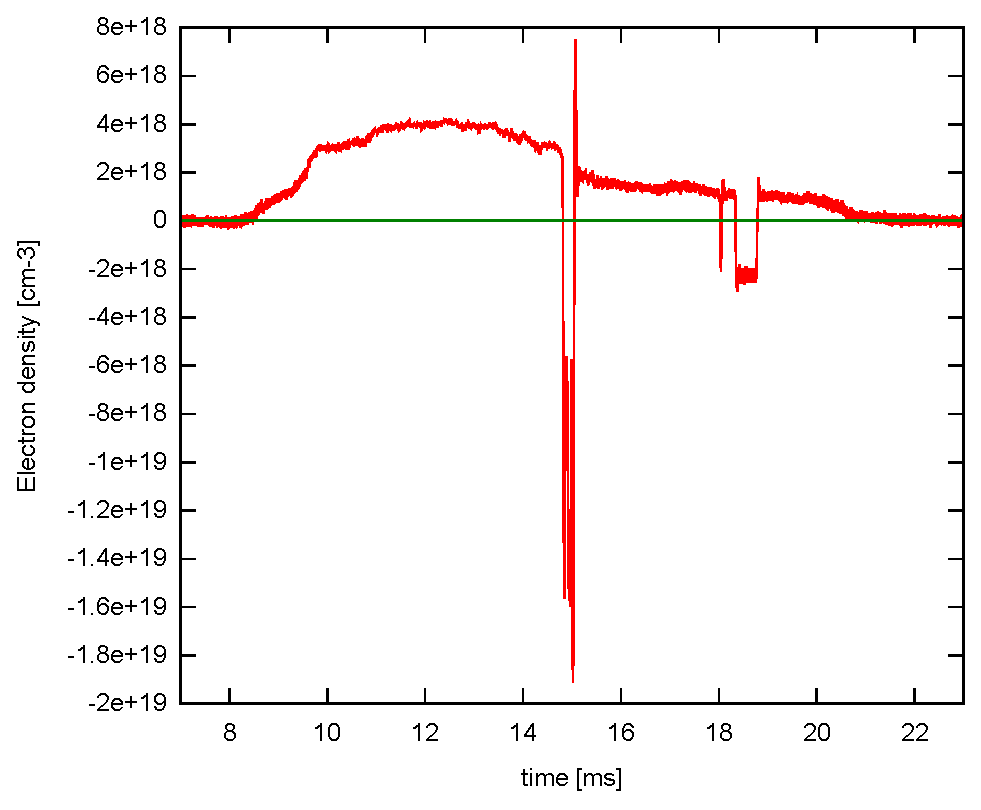
\includegraphics[width=.45\textwidth]{data.eps}
    \end{center}
    \caption{Electron density during discharge \# 5725}
    \label{fig:data}
\end{figure}

During most discharges several different disturbances have been observed as seen for example in Figure \ref{fig:data}. These regions are characterised by an increase or decrease in the frequency of the amplified sine wave signal which is interpreted as rapid increase or decrease of the phase shift by both of the methods of analysis.

These disturbances are assumed to be triggered by the behaviour of plasma during the discharge, because they occur usually only after the initial exponential rise in the density and do not occur while there is no plasma in the chamber. By increasing the temperature of the chamber which results in a better vacuum the stability of the plasma during the discharge is improved. The stability of the discharge appears to greatly affect the number of occurrences of the disturbances.

It is therefore hypothesized that there exists coupling of the diagnostic analysis hardware and the chamber through the waveguide system and it may be the event of plasma crashing on the wall of the chamber that triggers the disturbances.

However, it is not clear what the relationship between the triggering event and the change in the frequency is. The hypothesized coupling would most likely change the generated $f_{mod}$ and/or $\Delta f$ which could for example result in disrupting (\ref{eq:Df}) and making the triggering frequency obsolete. However, such scenarios fail to completely explain the disturbances.

In the future a different saw-tooth voltage and trigger signal generator with better grounding will be used to overcome the possible coupling. The plasma position stabilisation system, once fully operational, will be used to improve the stability of the discharge.\\

\noindent ACKNOWLEDGEMENTS: This project has been supervised by Ing. Vojtěch Svoboda %I wouldlike to thank... 
%------------------------------------


\begin{thebibliography}{99}

%\leftskip=-5pt \vspace{-0.3truecm}
\bibitem{mateju}
   MATĚJŮ, Michael.
   {\em Měření hustoty plazmatu metodami mikrovlnné interferometre. }
   FJFI, 2008. 44 s. Bakalářská práce. ČVUT, FJFI, Katedra fyziky. Dostupné z WWW: {\tt http://golem.fjfi.cvut.cz/files/students/
   BcTh/MatejuMichael.pdf}.
\end{thebibliography}


\end{document}
